\begin{frame}{Обратная динамика}{Цели раздела}
    \begin{block}{Задачи}
        \begin{enumerate}
            \item <+-> []
            \item <+-> Зачем использовать обратную динамику 
            \item <+-> Проблемы использования обратной динамики
            \item <+-> Пhименение PI-контроллера в обратой динамики
        \end{enumerate}
    \end{block}
\end{frame}

\begin{frame}{Обратная динамика}{Применение}
    \begin{block}{Схема}
        \center{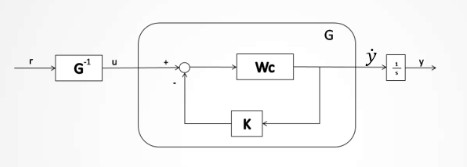
\includegraphics[width=11cm, height = 6cm]{../Оглавление/Part3/figures/ОД.jpg}}
    \end{block}
\end{frame}

\begin{frame}{Обратная динамика}{Проблемы использования}
    \begin{itemize}
        \item <+-> []
        \item <+-> [] \begin{block}{Важно}
            \begin{itemize}
                \item Порядок числителя выше порядка знаменателя 
                \item "Шаткая" робастность системы
            \end{itemize}
        \end{block}
        \begin{exampleblock}{Пример}
            $$G^{-1} = \frac{a_n p^k + a_{n-1} p^{k-1} + ... + a_0}{b_m p^{k-1} + b_{m-1} p^{k-2} + ... + b_0}$$
        \end{exampleblock}
    \end{itemize}
\end{frame}

\begin{frame}{Обратная динамика}{Робастность системы}
    \begin{block}{Схема}
        \center{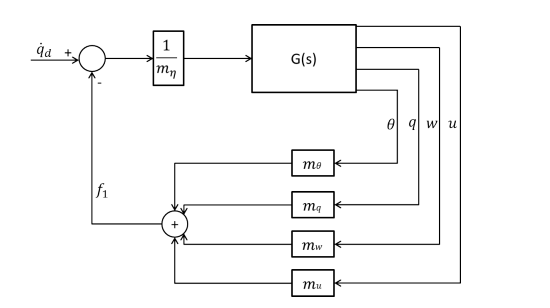
\includegraphics[width=11cm, height = 6cm]{../Оглавление/Part3/figures/Неполная схема СПС.png}}
    \end{block}
\end{frame}

\begin{frame}{Обратная динамика}{Робастность системы}
    \begin{block}{Результаты экспериментов}
        \center{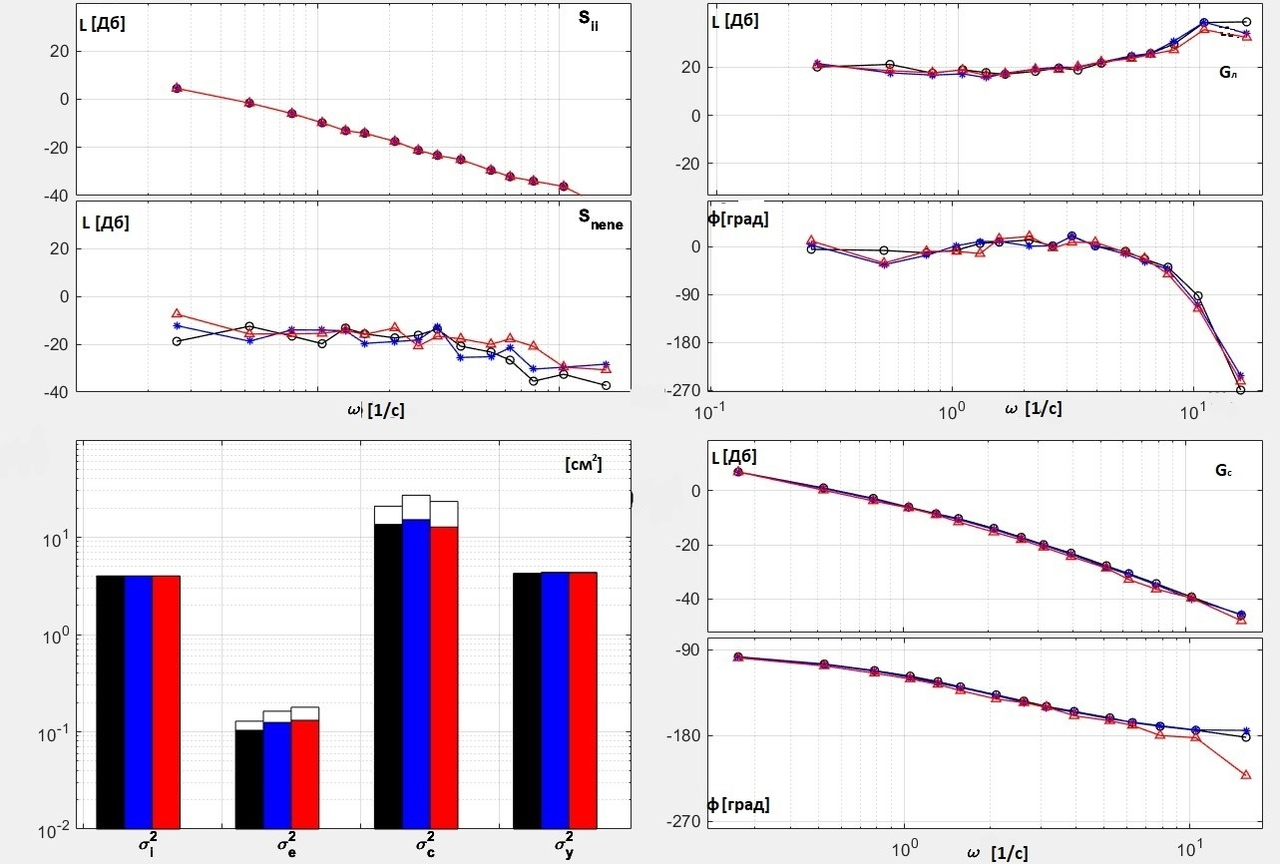
\includegraphics[width=11cm, height = 6cm]{../Оглавление/Part3/figures/Модель без PI.jpg}}
    \end{block}
\end{frame}

\begin{frame}{Обратная динамика}{Робастность системы}

\begin{table}[H]
    \begin{tabular}{|c|c|c|c|}
        \hline 
        № э.& $\sigma^2_e,$ см$^2$ & $\sigma^2_c$ см$^2$ & $n_e$ см$^2$ \\ \hline 
        1& 0.103 & 13.54 & 0.0254\\ \hline
        2& 0.125 & 15.14  & 0.037 \\ \hline
        3& 0.131 & 12.74 & 0.047\\ \hline

    \end{tabular}
\end{table}
\end{frame}
 
\begin{frame}{Обратная динамика}{Робастность системы}
\begin{table}[H]
    \begin{tabular}{|c|c|c|c|c|}
        \hline 
        № э.&Нули & Полюса & $\xi$ & $\omega_c$, 1/c \\ \hline 
        1& -2 & - & 1.0 &0.5 \\ \hline
        & -1.9392 & -0.7537  &  & 1.59 $\cdot 10^{-4}$\\ 
        2& -0.7473 & -0.0161  &1.0 & 1.64 $\cdot 10^{-2}$\\ 
        & -0.0164 &  0 & &7.47 $\cdot 10^{-1}$\\ 
        & 0 &   &  &1.94 \\ \hline 
        & -1.8207 & 0.8255 & &0\\ 
        3& -0.8033 & -0.0177 & 1.0&1.85 $\cdot 10^{-2}$\\ 
        & -0.0185 & 0 & &8.03 $\cdot 10^{-1}$ \\ 
        & 0 &  &  &1.82 \\ \hline
    \end{tabular}
\end{table}

\end{frame}

\begin{frame}{Обратная динамика}{Робастность системы}
    \begin{block}{Результаты при изменении динамик самолёта на 80 \%}
        \center{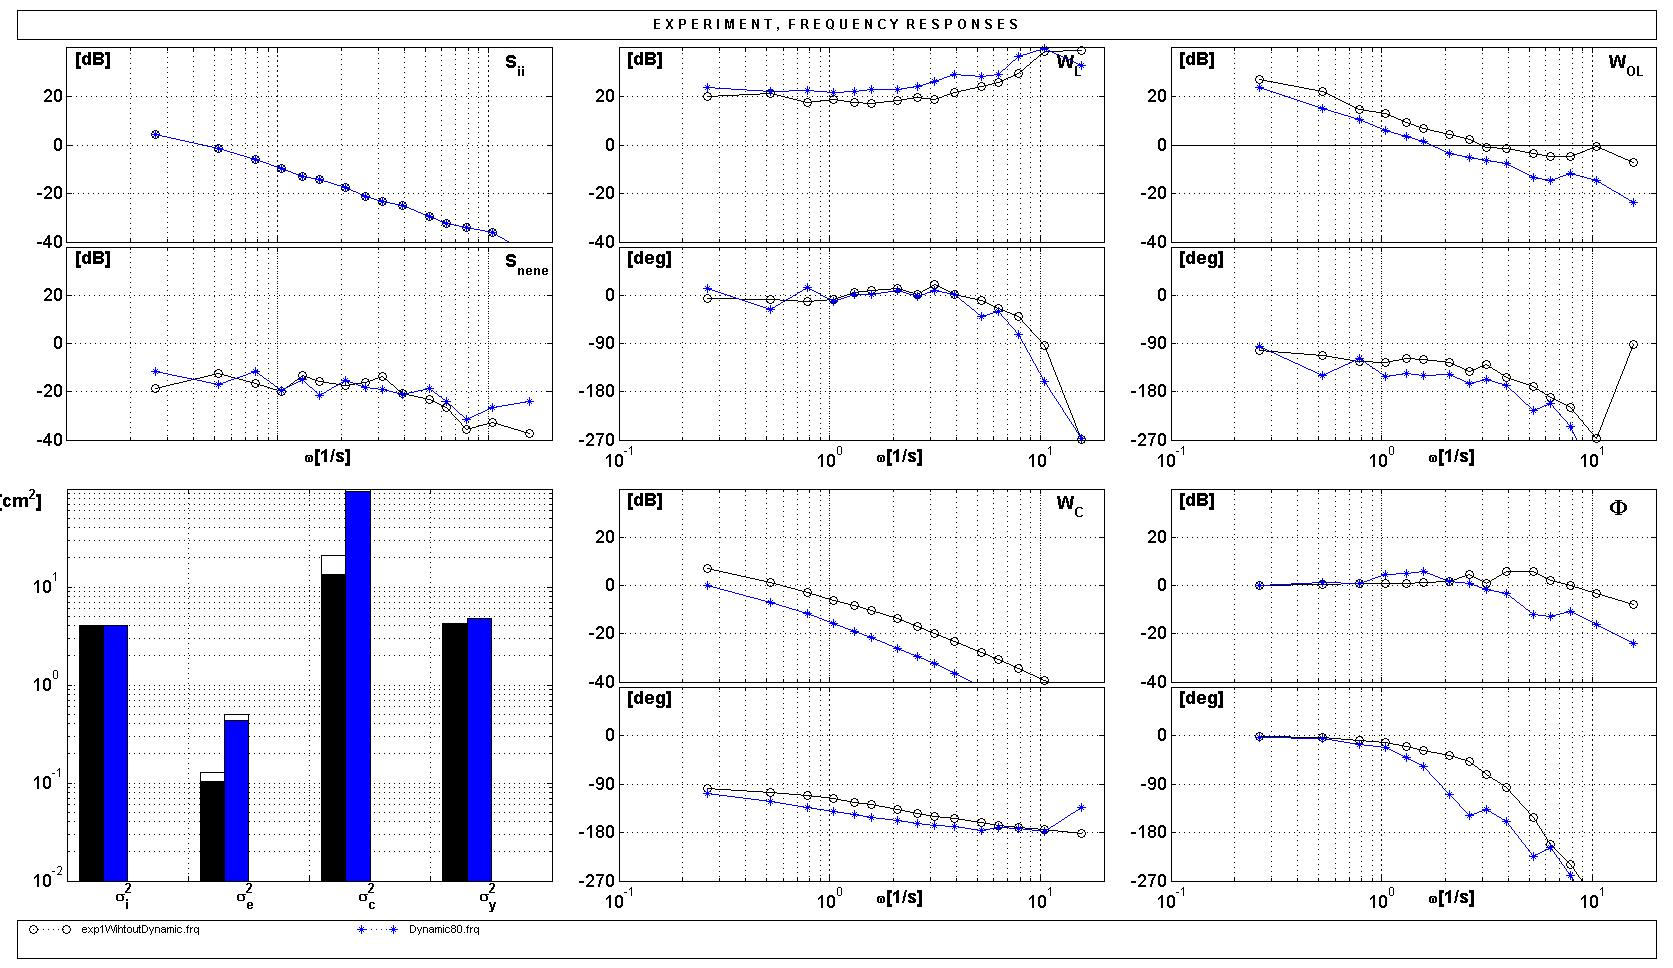
\includegraphics[width=11cm, height = 6cm]{../Оглавление/Part3/figures/testo2.jpg}}
    \end{block}
\end{frame}

\begin{frame}{Обратная динамика}{Улучшение робасности с применением PI-контроллера}
    \begin{block}{Схема}
        \center{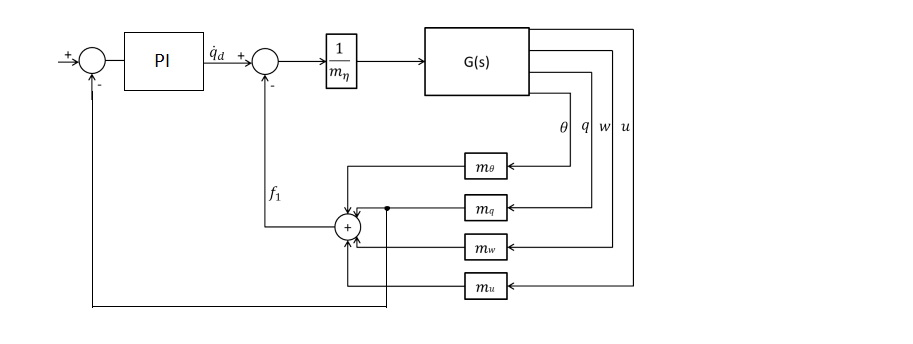
\includegraphics[width=15cm, height = 6cm]{../Оглавление/Part3/figures/Полная схема СПС.png}}
    \end{block}
\end{frame}

\begin{frame}{Обратная динамика}{Улучшение робасности с применением PI-контроллера}
    \begin{block}{Результаты экспериментов}
        \center{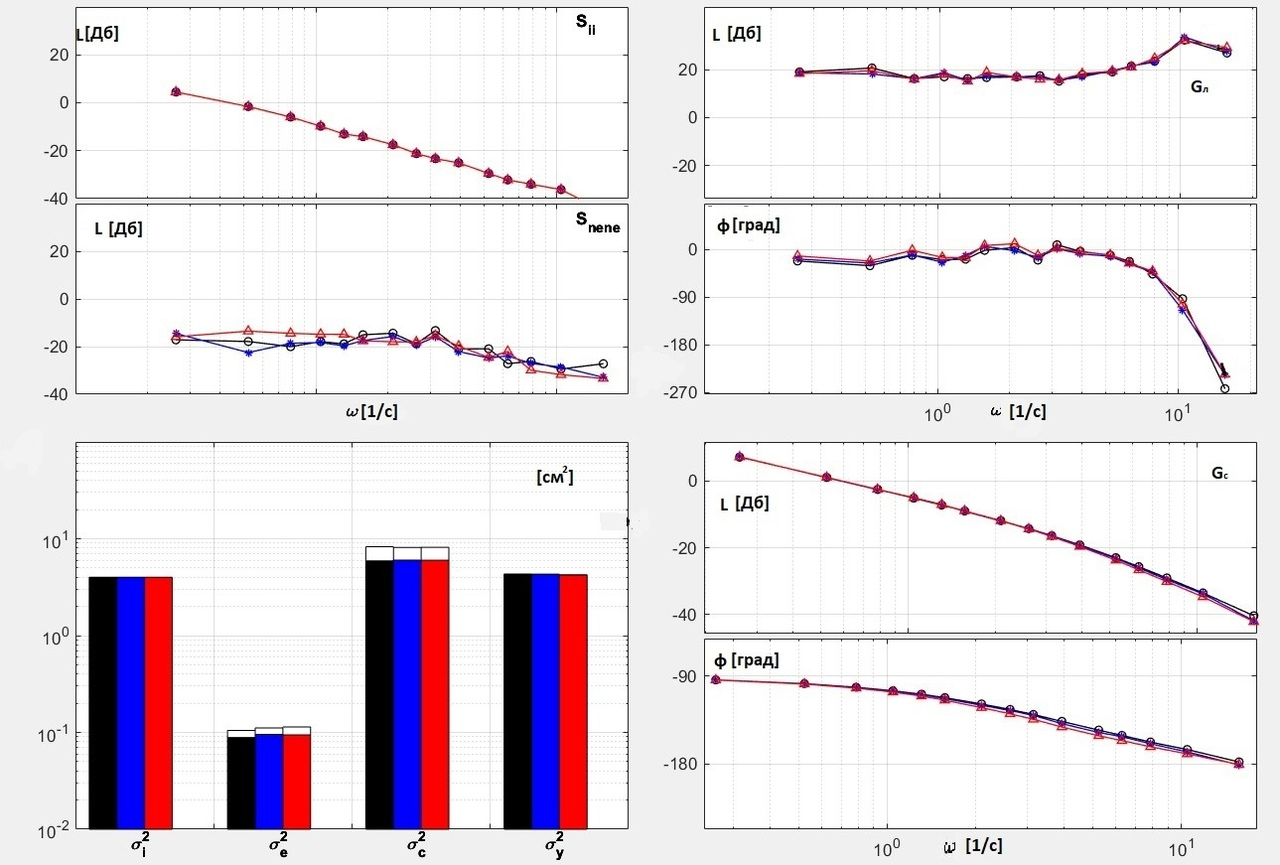
\includegraphics[width=11cm, height = 6cm]{../Оглавление/Part3/figures/Модель с PI.jpg}}
    \end{block}
\end{frame}


\begin{frame}{Обратная динамика}{Робастность системы}

\begin{table}[H]
    \begin{tabular}{|c|c|c|c|}
        \hline 
        № э.& $\sigma^2_e,$ см$^2$ & $\sigma^2_c$ см$^2$ & $n_e$ см$^2$ \\ \hline 
        1& 0.0886 & 5.913 & 0.01611\\ \hline
        2& 0.0952 & 6.01  & 0.01591 \\ \hline
        3& 0.0943 & 6.004 & 0.01712\\ \hline

    \end{tabular}
\end{table}
\end{frame}
 
\begin{frame}{Обратная динамика}{Робастность системы}
\begin{table}[H]
    \begin{tabular}{|c|c|c|c|c|}
        \hline 
        № э.&Полюса & Нули & $\xi$ & $\omega_c$, 1/c \\ \hline 
        1& -3.0000 + 1.0000$i$ & -2.5 & 0.95 & 3.16\\ 
        & -3.0000 - 1.0000$i$ &   &  &  \\ \hline
        2& -2.8660 + 1.1287$i$ & -0.0161  & 1.0 &  0\\ 
        & -2.8660 - 1.1287$i$ &  -0.7537 &1.0 & 1.61$\cdot 10^{-2}$\\ 
        & -0.7547 + 0.0000$i$ &  -2.5000 & 1.0 & 7.51 $\cdot 10^{-2}$\\ 
        & 0 & 0.0000 & 0.93& 3.08 \\ 
        & -0.0161 + 0.0000$i$ &  & 0.93 &  \\ \hline 
        3& -2.5975 + 1.3096$i$ & -0.0177 & 1 & 0\\ 
        & -2.5975 - 1.3096$i$ & -0.8255 & 1& 1.77 $\cdot 10^{-2}$ \\ 
        & -0.8292 + 0.0000$i$ & -2.5000 & 1 & 8.29 $\cdot 10^{-1}$\\ 
        & 0 & 0 & 0.893 & 2.91 \\ 
        & -0.0177 + 0.0000$i$ &  &  &  \\ \hline 
    \end{tabular}
\end{table}

\end{frame}